\section{随机累计与变量变换}
\label{sec:ctsp-stochastic-integration}

离散章的鞅变换$\sum_kH_k(M_{k+1}-M_k)$把每一步开始时选定的权重乘到下一步的噪声上，再累计起来；只要权重不偷看下一步，累计量仍是鞅。本节把这个运算推广到连续时间：给定被积过程$H$和驱动（时间、计数或Brownian运动），定义累计量$\int_0^tH_s\,\mathrm dX_s$，再计算状态函数$f(X_t)$怎样变化。这里被积过程与驱动都是事先给定的；系数依赖未知状态、需要求解的情形留给下一节。

三类驱动的处理方式不同。时间与有限次跳跃可以逐路径累计；Brownian路径的总变差无限，必须借助均方误差在$L^2$中构造积分。变量变换同样分化：有限变差路径遵守普通链式法则，Brownian路径的二次变差留下一个二阶修正，跳跃则保留完整的有限差。

\subsection{时间积分与跳跃积分}
\label{sec:ctsp-time-jump-integrals}

\paragraph{逐路径的时间积分}
最简单的累计是对时间积分。设$b$渐进可测，并且对每个$t$，$\int_0^t|b_s|\,\mathrm ds<\infty$几乎必然。对每条路径，$A_t=\int_0^tb_s\,\mathrm ds$是普通的Lebesgue积分；渐进可测性保证$A_t$是$\mathcal F_t$可测的，于是$A$是连续适应过程。取期望并交换积分次序时，用的是Fubini--Tonelli定理，需要$\mathbb E\int_0^t|b_s|\,\mathrm ds<\infty$；这些积分工具见\BookChapterRef{chap:integration}{卷二“积分”章}。

$A$还具有\term{有限变差}（finite variation）：任一分割上$\sum_i|A_{t_{i+1}}-A_{t_i}|\leq\int_0^t|b_s|\,\mathrm ds$。有限变差的路径可以作为Stieltjes积分的积分器，并且它的平方增量和趋于零，这两点在后面区分不同驱动时都会用到。

\paragraph{计数积分与左极限}
对计数过程$N$，累计只发生在跳跃时刻。对有限值的过程$H$，自然的定义是
\begin{equation}
  \int_0^tH_s\,\mathrm dN_s=\sum_{k:\,T_k\leq t}H_{T_k}.
  \label{eq:ctsp-counting-integral}
\end{equation}
有限时段内只有有限次跳跃，这个和逐路径有定义。问题在于$H$在跳跃时刻取哪个值。若$H$可预测，$H_{T_k}$只依赖$T_k$之前的信息，可以理解为“事件发生前就定好的单次影响”；若$H_s=g(X_{s-})$，取的是跳前状态。

左右极限的差别可以直接算出来。以单位跳跃的计数过程为例，第$k$次事件时$N_{T_k-}=k-1$，$N_{T_k}=k$，于是
\[
  \int_0^tN_{s-}\,\mathrm dN_s=\sum_{k=1}^{N_t}(k-1)=\frac{N_t(N_t-1)}2,\qquad
  \sum_{k=1}^{N_t}N_{T_k}=\frac{N_t(N_t+1)}2 ,
\]
两者相差$N_t$。下面会看到，只有前者与补偿结构相容。

\paragraph{补偿积分的均值与等距}
设$N$是速率$\lambda$的Poisson过程，$H$是可预测过程。扣除平均事件量，定义补偿积分
\begin{equation}
  \int_0^tH_s\,\mathrm d\widetilde N_s=\sum_{k:\,T_k\leq t}H_{T_k}-\lambda\int_0^tH_s\,\mathrm ds .
  \label{eq:ctsp-compensated-integral}
\end{equation}

\begin{theorem}[补偿积分的均值与二阶矩]
  \label{thm:ctsp-poisson-integral}
  设$H$可预测。若\allowbreak$\mathbb E\int_0^T|H_s|\,\mathrm ds<\infty$，则
  \[
    \mathbb E\int_0^TH_s\,\mathrm dN_s=\lambda\,\mathbb E\int_0^TH_s\,\mathrm ds,
  \]
  于是补偿积分的期望为零。若$\mathbb E\int_0^TH_s^2\,\mathrm ds<\infty$，则补偿积分在$[0,T]$上是平方可积鞅，并且
  \begin{equation}
    \mathbb E\Bigl(\int_0^TH_s\,\mathrm d\widetilde N_s\Bigr)^2=\lambda\,\mathbb E\int_0^TH_s^2\,\mathrm ds .
    \label{eq:ctsp-poisson-isometry}
  \end{equation}
\end{theorem}

\begin{proof}
先取简单可预测过程$H_s=\sum_iH_i\mathbb I_{(t_i,t_{i+1}]}(s)$，$H_i$有界且$\mathcal F_{t_i}$可测。此时$\int H\,\mathrm d\widetilde N=\sum_iH_i\Delta\widetilde N_i$，其中$\Delta\widetilde N_i=\widetilde N_{t_{i+1}}-\widetilde N_{t_i}$独立于$\mathcal F_{t_i}$，均值为零，方差为$\lambda\Delta t_i$。每一项的期望$\mathbb E[H_i\,\mathbb E(\Delta\widetilde N_i\mid\mathcal F_{t_i})]=0$；平方展开后，$i<j$的交叉项先对$\mathcal F_{t_j}$取条件期望即为零，对角项给出$\lambda\Delta t_i\,\mathbb EH_i^2$。这证明了简单过程的两个等式，鞅性质由同样的条件期望计算得到。

一般情形用逼近完成。可预测$\sigma$代数由矩形$(s,u]\times A$（$A\in\mathcal F_s$）生成，而矩形指示过程正是简单可预测过程；对可预测集合$B\subseteq(0,T]\times\Omega$，两个有限测度$B\mapsto\mathbb E\int\mathbb I_B\,\mathrm dN$与$B\mapsto\lambda\mathbb E\int\mathbb I_B\,\mathrm ds$在矩形上相等，矩形族对有限交封闭，由单调类定理它们在整个可预测$\sigma$代数上相等。再用简单函数逼近非负可预测$H$并取单调极限，得到第一式；有符号情形对正负部分别使用。二阶等式先对简单过程成立，再按等距在$L^2$中延拓，延拓结果与式~\eqref{eq:ctsp-compensated-integral}的逐路径定义一致，因为第一式保证了两者之差的期望绝对值为零。
\end{proof}

可预测性不是技术细节。若把跳后的$N_s$当作系数，
\[
  \begin{aligned}
    \mathbb E\sum_{k\leq N_t}N_{T_k}&=\mathbb E\frac{N_t(N_t+1)}2=\frac{(\lambda t)^2}2+\lambda t,\\
    \lambda\,\mathbb E\int_0^tN_s\,\mathrm ds&=\lambda\int_0^t\lambda s\,\mathrm ds=\frac{(\lambda t)^2}2,
  \end{aligned}
\]
两者之差为$\lambda t\neq0$：声称的“补偿积分”有正的平均漂移。原因是跳后的系数在事件发生的那一刻把这次事件也算了进去。改用$N_{s-}$，$\mathbb EN_t(N_t-1)/2=(\lambda t)^2/2$，差恰好消失。

若只知道每个有限$T$上$\int_0^TH_s^2\,\mathrm ds<\infty$几乎必然，可以取停时$\rho_n=\inf\{t:\lambda\int_0^tH_s^2\,\mathrm ds\geq n\}\wedge n$。累计平方连续、适应且非减，所以$\rho_n$是停时；停止后的被积过程满足定理的二阶条件，补偿积分因而是局部鞅。去掉截断后能否取零均值，仍需另行检查可积性。

\begin{example}[按跳前状态计费]
  \label{ex:ctsp-predictable-fee}
  一台设备在每次故障时产生维修费用，费用等于故障前已累计的故障次数加一，即$H_s=N_{s-}+1$。$[0,t]$上的总费用为$\int_0^t(N_{s-}+1)\,\mathrm dN_s=N_t(N_t+1)/2$，其期望由定理~\ref{thm:ctsp-poisson-integral}给出：$\lambda\int_0^t(\lambda s+1)\,\mathrm ds=(\lambda t)^2/2+\lambda t$。直接用$\mathbb EN_t^2=(\lambda t)^2+\lambda t$计算，结果相同。这里系数可以依赖全部过去，只要不依赖当次事件。
\end{example}

\subsection{Brownian积分}
\label{sec:ctsp-brownian-integral}

\paragraph{简单可预测过程的累计}
现在把驱动换成Brownian运动。第~\ref{sec:ctsp-brownian}节说明它的路径总变差无限，不能逐路径地定义Stieltjes积分；但离散鞅变换提示了另一条路：先对在有限个时刻改变取值的被积过程定义累计，再利用均方误差把定义推广出去。

设$0=t_0<t_1<\cdots<t_n=T$，$H_i\in L^2(\mathcal F_{t_i})$，称$H_s=\sum_iH_i\mathbb I_{(t_i,t_{i+1}]}(s)$为简单可预测过程。系数在每段开始时确定，可以依赖开始以前的全部历史，但不能借用本段的Brownian增量。定义
\begin{equation}
  \int_0^tH_s\,\mathrm dW_s=\sum_iH_i\bigl(W_{t\wedge t_{i+1}}-W_{t\wedge t_i}\bigr).
  \label{eq:ctsp-simple-ito}
\end{equation}

\begin{lemma}[简单过程的Itô等距]
  \label{lem:ctsp-simple-isometry}
  对简单可预测过程$H$，$M_t=\int_0^tH_s\,\mathrm dW_s$是连续的平方可积鞅，并且
  \[
    \mathbb E\Bigl(\int_0^TH_s\,\mathrm dW_s\Bigr)^2=\mathbb E\int_0^TH_s^2\,\mathrm ds .
  \]
\end{lemma}

\begin{proof}
路径连续由$W$的连续性直接得到。对$s<t$，起点不早于$s$的每一段都满足$\mathbb E[H_i\Delta W_i\mid\mathcal F_s]=\mathbb E\{H_i\,\mathbb E[\Delta W_i\mid\mathcal F_{t_i}]\mid\mathcal F_s\}=0$，包含$s$的那一段用已知系数乘以$s$之后的零均值增量，同样没有条件漂移，所以$M$是鞅。平方展开时，对$i<j$，$H_iH_j\Delta W_i$是$\mathcal F_{t_j}$可测的，而$\Delta W_j$独立于$\mathcal F_{t_j}$且均值为零，交叉项期望为零；对角项为$\mathbb E[H_i^2\,\mathbb E((\Delta W_i)^2\mid\mathcal F_{t_i})]=\Delta t_i\,\mathbb EH_i^2$。逐项相加即得等距。交叉乘积的可积性由Cauchy--Schwarz不等式保证。
\end{proof}

\paragraph{$L^2$延拓}
等距说明，积分把被积过程空间中的距离原样搬到随机变量空间中。记$\mathcal H^2_T$为满足$\mathbb E\int_0^TH_s^2\,\mathrm ds<\infty$的可预测过程全体（几乎处处相等者视为同一元素），范数为$\|H\|^2_{\mathcal H^2}=\mathbb E\int_0^TH_s^2\,\mathrm ds$。它是$[0,T]\times\Omega$上关于测度$\mathrm ds\otimes\mathbb P$、限制在可预测$\sigma$代数上的$L^2$空间，因而是完备的Hilbert空间；$L^2$空间完备性的证明见\BookChapterRef{chap:function-spaces}{卷二“函数空间”章}。简单可预测过程在$\mathcal H^2_T$中稠密\scite{math-oksendal2003sde}：对连续有界的适应过程，取左端点的阶梯逼近，由路径连续与控制收敛即在该范数下收敛；一般情形再由连续过程逼近。

\begin{theorem}[Itô积分]
  \label{thm:ctsp-ito-integral}
  对$H\in\mathcal H^2_T$，取简单可预测过程$H^{(n)}\to H$于$\mathcal H^2_T$。则$\int_0^TH^{(n)}_s\,\mathrm dW_s$在$L^2(\mathbb P)$中收敛，极限不依赖逼近列的选择，记为$\int_0^TH_s\,\mathrm dW_s$，称为\term{Itô积分}（Itô integral）。作为$t\in[0,T]$的函数，它有连续版本，是平方可积鞅，并满足\term{Itô等距}
  \begin{equation}
    \mathbb E\Bigl(\int_0^TH_s\,\mathrm dW_s\Bigr)^2=\mathbb E\int_0^TH_s^2\,\mathrm ds .
    \label{eq:ctsp-ito-isometry}
  \end{equation}
\end{theorem}

\begin{proof}
由引理~\ref{lem:ctsp-simple-isometry}，$\|\int H^{(n)}\mathrm dW-\int H^{(m)}\mathrm dW\|_{L^2}=\|H^{(n)}-H^{(m)}\|_{\mathcal H^2}$，所以积分列是$L^2$中的Cauchy列，由完备性收敛；两列逼近交错排列仍是Cauchy列，极限唯一。等距在极限中保持。条件期望是$L^2$上的压缩，鞅等式在极限中保持。对连续版本，把Doob的$L^2$最大不等式用于差$\int H^{(n)}\mathrm dW-\int H^{(m)}\mathrm dW$，得到$\mathbb E\sup_{t\leq T}|\cdot|^2\leq4\|H^{(n)}-H^{(m)}\|^2_{\mathcal H^2}$；选子列使这些量可求和，Borel--Cantelli引理给出几乎必然的一致收敛，连续函数的一致极限仍连续。
\end{proof}

若只有$\int_0^TH_s^2\,\mathrm ds<\infty$几乎必然，令$\rho_n=\inf\{t:\int_0^tH_s^2\,\mathrm ds\geq n\}\wedge T$。停止后的被积过程属于$\mathcal H^2_T$，各截断上的积分在共同时段上一致，拼接成一个连续的局部鞅。本章说$\int H\,\mathrm dW$时，默认被积过程满足这一局部条件。

\paragraph{两个直接计算}
确定性被积函数给出最简单的例子。若$f$是$[0,T]$上的平方可积确定函数，简单逼近的每一项都是独立高斯增量的线性组合，$L^2$极限仍是高斯变量，所以
\[
  \int_0^Tf(s)\,\mathrm dW_s\sim\mathcal N\Bigl(0,\int_0^Tf(s)^2\,\mathrm ds\Bigr).
\]
这一结论将用于线性随机微分方程的解。

被积过程是Brownian运动本身时，左端点取样的Riemann和可以直接求极限。由恒等式$W_{t_i}\Delta W_i=\frac12[W_{t_{i+1}}^2-W_{t_i}^2-(\Delta W_i)^2]$，
\[
  \sum_iW_{t_i}\Delta W_i=\frac12W_T^2-\frac12\sum_i(\Delta W_i)^2\longrightarrow\frac12(W_T^2-T)\qquad\text{于 }L^2,
\]
最后一步用了定理~\ref{thm:ctsp-brownian-qv}。于是
\begin{equation}
  \int_0^TW_s\,\mathrm dW_s=\frac12(W_T^2-T).
  \label{eq:ctsp-int-w-dw}
\end{equation}
普通微积分会给出$\frac12W_T^2$，多出来的$-\frac T2$就是二次变差留下的痕迹。作为核对，等距给出方差$\int_0^T\mathbb EW_s^2\,\mathrm ds=T^2/2$，而$\operatorname{Var}((W_T^2-T)/2)=\operatorname{Var}(W_T^2)/4=T^2/2$，二者一致。

\paragraph{Itô过程}
把时间积分与Brownian积分合在一起，就得到后面换元公式和随机微分方程的基本对象。

\begin{definition}[Itô过程]
  \label{def:ctsp-ito-process}
  设$\bm W$是$m$维标准Brownian运动，$\bm X_0$是$\mathcal F_0$可测的$\mathbb R^d$值随机向量，$\bm b_t\in\mathbb R^d$渐进可测，$\bm\sigma_t\in\mathbb R^{d\times m}$可预测，并且每个有限$T$上$\int_0^T(\|\bm b_t\|_2+\|\bm\sigma_t\|_{\mathrm F}^2)\,\mathrm dt<\infty$几乎必然。称
  \[
    \bm X_t=\bm X_0+\int_0^t\bm b_s\,\mathrm ds+\int_0^t\bm\sigma_s\,\mathrm d\bm W_s
  \]
  为\term{Itô过程}（Itô process），记作$\mathrm d\bm X_t=\bm b_t\,\mathrm dt+\bm\sigma_t\,\mathrm d\bm W_t$。$\bm b$称为漂移，$\bm\sigma$称为扩散系数；向量积分逐分量理解，$(\int\bm\sigma\,\mathrm d\bm W)_i=\sum_j\int\sigma_{i,j}\,\mathrm dW^{(j)}$。
\end{definition}

记号$\mathrm d\bm X_t$只是积分方程的简写，并不断言$\bm X$可微。Itô过程是有限变差的漂移部分与连续局部鞅之和；这种分解是唯一的，因为一个既是有限变差又是连续局部鞅的过程只能是常数\scite{math-kallenberg2021probability}。

\subsection{二次变差与Itô公式}
\label{sec:ctsp-ito-formula}

\paragraph{从离散平方恒等式出发}
要计算状态函数$f(X_t)$的变化，先回到一条分割上的Taylor展开：
\[
  f(X_t)-f(X_0)=\sum_if'(X_{t_i})\Delta X_i+\frac12\sum_if''(\xi_i)(\Delta X_i)^2 ,
\]
其中$\xi_i$介于$X_{t_i}$与$X_{t_{i+1}}$之间。若$X$是光滑或有限变差的路径，第二个和被$\max_i|\Delta X_i|\cdot\sum_i|\Delta X_i|$控制，趋于零，留下的就是普通链式法则。若$X=W$，平方增量和不消失，第二个和趋于$\frac12\int_0^tf''(W_s)\,\mathrm ds$。这正是Itô公式中二阶修正项的来源。

一般Itô过程的平方增量和需要保留扩散系数。沿网格宽度趋零的分割，
\begin{equation}
  [X^{(i)},X^{(j)}]_t=\lim\sum_k\Delta X^{(i)}_k\Delta X^{(j)}_k=\int_0^t(\bm\sigma_s\bm\sigma_s^\top)_{i,j}\,\mathrm ds\qquad\text{依概率},
  \label{eq:ctsp-ito-covariation}
\end{equation}
称为\term{二次协变差}（quadratic covariation）。漂移部分有限变差，不贡献二次变差；独立Brownian分量的交叉乘积和趋于零，相同分量的平方和趋于时间长度。例如$X=2W$时$[X]_t=4t$，不是$t$。一个有用的形式记忆规则是
\[
  \mathrm dt\cdot\mathrm dt=0,\qquad\mathrm dt\cdot\mathrm dW^{(j)}=0,\qquad\mathrm dW^{(i)}\cdot\mathrm dW^{(j)}=\delta_{i,j}\,\mathrm dt,
\]
它概括的是上述累计量的阶，不能替代可预测性与极限论证。

\paragraph{Itô公式}
下面的定理同时允许被变换的函数显含时间。记$C^{2,1}(\mathbb R^d\times[0,\infty))$为对状态变量二阶、对时间变量一阶连续可微的函数$V(t,\bm x)$全体，即$\partial_tV$、$\nabla V$、$\nabla^2V$都存在且关于$(t,\bm x)$连续。

\begin{theorem}[Itô公式]
  \label{thm:ctsp-ito-formula}
  设$\bm X$是定义~\ref{def:ctsp-ito-process}中的Itô过程，$V\in C^{2,1}(\mathbb R^d\times[0,\infty))$。则存在概率为一的事件，在其上对所有$t\geq0$同时有
  \begin{equation}
    \begin{aligned}
      V(t,\bm X_t)-V(0,\bm X_0)
      ={}&\int_0^t\Bigl[\partial_sV+\nabla V^\top\bm b_s+\tfrac12\operatorname{tr}\bigl(\bm\sigma_s\bm\sigma_s^\top\nabla^2V\bigr)\Bigr]\,\mathrm ds\\
      &+\int_0^t\nabla V^\top\bm\sigma_s\,\mathrm d\bm W_s ,
    \end{aligned}
    \label{eq:ctsp-ito-formula}
  \end{equation}
  其中$\partial_sV,\nabla V,\nabla^2V$都在$(s,\bm X_s)$处取值。微分记号写作
  \[
    \mathrm dV(t,\bm X_t)=\Bigl[\partial_tV+\nabla V^\top\bm b_t+\tfrac12\operatorname{tr}(\bm\sigma_t\bm\sigma_t^\top\nabla^2V)\Bigr]\mathrm dt+\nabla V^\top\bm\sigma_t\,\mathrm d\bm W_t .
  \]
\end{theorem}

式~\eqref{eq:ctsp-ito-formula}称为\term{Itô公式}（Itô formula）。公式的右端分成两部分：时间积分是$V(t,\bm X_t)$的漂移，它比普通链式法则多出$\frac12\operatorname{tr}(\bm\sigma\bm\sigma^\top\nabla^2V)$；随机积分是局部鞅。公式本身逐路径成立，但对它取期望时，随机积分项只是局部鞅，期望为零还需要额外条件，例如$\mathbb E\int_0^t\|\bm\sigma_s^\top\nabla V(s,\bm X_s)\|_2^2\,\mathrm ds<\infty$。

\paragraph{为什么二阶项留下而其余高阶项消失}
完整证明见Øksendal的随机微分方程教材第4章\scite{math-oksendal2003sde}。这里说明各项的去向，以免把二阶修正当作需要死记的规则。先用停时把$\bm X$截在有界区域内、并使系数有界，再在分割上对$V$作Taylor展开到时间一阶、空间二阶。

对时间与空间的一阶项，左端点取值的和分别收敛到$\int\partial_sV\,\mathrm ds$、$\int\nabla V^\top\bm b\,\mathrm ds$与随机积分$\int\nabla V^\top\bm\sigma\,\mathrm d\bm W$；后者正是Itô积分的定义方式，冻结左端点的误差由Itô等距控制。二阶项中，漂移与漂移、漂移与噪声的乘积和分别是$O(|\pi|)$与$O(|\pi|^{1/2})$量级，趋于零；噪声与噪声的乘积和则趋于二次协变差。关键估计是：对有界的$\mathcal F_{t_i}$可测权重$c_i$，
\[
  \mathbb E\Bigl|\sum_ic_i\bigl[(\Delta W_i)^2-\Delta t_i\bigr]\Bigr|^2=2\sum_i\mathbb E[c_i^2](\Delta t_i)^2\leq2\max_i\|c_i\|_\infty^2\,T|\pi| ,
\]
因为不同$i$的项在条件期望下正交，每一项的条件方差为$2(\Delta t_i)^2$。所以加权平方增量和收敛到加权时间积分，而不是零。三阶以上的余项被$\omega(\max_i\|\Delta\bm X_i\|)\sum_i\|\Delta\bm X_i\|^2$控制，其中$\omega$是二阶导数在紧集上的连续模，路径连续使第一个因子趋零，第二个因子依概率有界。最后令停时递增，去掉截断。

\paragraph{计算示例}
几个计算展示公式的用法，每一个都可以与已有结论核对。
\begin{enumerate}
  \item 取$V(x)=x^2$、$X=W$：$\mathrm d(W_t^2)=2W_t\,\mathrm dW_t+\mathrm dt$，积分即得式~\eqref{eq:ctsp-int-w-dw}。
  \item 取$V(x)=x^4$、$X=W$：$\mathrm d(W_t^4)=4W_t^3\,\mathrm dW_t+6W_t^2\,\mathrm dt$。被积过程$4W^3$满足$\mathbb E\int_0^t16W_s^6\,\mathrm ds<\infty$，随机积分是真鞅，取期望得$\mathbb EW_t^4=6\int_0^ts\,\mathrm ds=3t^2$，与正态四阶矩一致。
  \item 取含时间的$V(t,x)=\exp(\theta x-\theta^2t/2)$、$X=W$：$\partial_tV+\frac12\partial_{xx}V=(-\frac{\theta^2}2+\frac{\theta^2}2)V=0$，所以$\mathrm dV(t,W_t)=\theta V(t,W_t)\,\mathrm dW_t$，漂移恰好消失。这从另一角度说明了第~\ref{sec:ctsp-continuous-martingales}节的指数鞅为什么需要因子$e^{-\theta^2t/2}$。
\end{enumerate}

两个Itô过程的乘积是另一个常用特例。对$V(x,y)=xy$使用二维公式，$\nabla^2V$只有非对角元$1$，得到
\begin{equation}
  \mathrm d(X_tY_t)=X_t\,\mathrm dY_t+Y_t\,\mathrm dX_t+\mathrm d[X,Y]_t .
  \label{eq:ctsp-product-rule}
\end{equation}
若其中一个因子有限变差（例如确定函数$e^{\lambda t}$），交叉变差为零，乘积法则与普通微积分相同。下一节求解线性方程时，正是利用这一点构造积分因子。

\paragraph{有限活动跳跃的Itô公式}
最后加入计数驱动。设
\[
  \bm X_t=\bm X_0+\int_0^t\bm b_s\,\mathrm ds+\int_0^t\bm\sigma_s\,\mathrm d\bm W_s+\int_0^t\bm\gamma_s\,\mathrm dN_s ,
\]
其中$N$是速率$\lambda$的Poisson过程，$\bm\gamma$可预测且有限。路径在相邻事件之间是连续Itô过程，在事件时刻$T_k$跳$\Delta\bm X_{T_k}=\bm\gamma_{T_k}$。在相邻事件之间使用定理~\ref{thm:ctsp-ito-formula}，在每个事件处加上$V$的精确增量，再把有限个片段首尾相接，得到：对$V\in C^{2,1}$，
\begin{equation}
  \begin{aligned}
    V(t,\bm X_t)-V(0,\bm X_0)
    ={}&\int_0^t\Bigl[\partial_sV+\nabla V^\top\bm b_s+\tfrac12\operatorname{tr}(\bm\sigma_s\bm\sigma_s^\top\nabla^2V)\Bigr](s,\bm X_{s-})\,\mathrm ds\\
    &+\int_0^t\nabla V(s,\bm X_{s-})^\top\bm\sigma_s\,\mathrm d\bm W_s\\
    &+\int_0^t\bigl[V(s,\bm X_{s-}+\bm\gamma_s)-V(s,\bm X_{s-})\bigr]\,\mathrm dN_s .
  \end{aligned}
  \label{eq:ctsp-jump-ito}
\end{equation}
跳跃项保留的是完整的有限差$V(\bm x+\bm\gamma)-V(\bm x)$，而不是Taylor展开到二阶的近似；跳幅不必很小，推导也不需要它很小。把最后一项写成补偿形式，$\mathrm dN_s=\mathrm d\widetilde N_s+\lambda\,\mathrm ds$，漂移中就多出$\lambda[V(s,\bm X_{s-}+\bm\gamma_s)-V(s,\bm X_{s-})]$，其余部分是零均值的跳跃鞅项（在相应可积条件下）。

\begin{example}[计数平方的修正]
  \label{ex:ctsp-poisson-square}
  取$X=N$、$V(x)=x^2$。每次事件使平方增加$(N_{s-}+1)^2-N_{s-}^2=2N_{s-}+1$，所以$N_t^2=\int_0^t(2N_{s-}+1)\,\mathrm dN_s$。由定理~\ref{thm:ctsp-poisson-integral}，$\mathbb EN_t^2=\lambda\int_0^t(2\lambda s+1)\,\mathrm ds=(\lambda t)^2+\lambda t$，与Poisson分布的二阶矩一致。Brownian平方的修正是连续的$t$，计数平方的修正是随机的事件数$N_t$；后者的平均才是$\lambda t$。
\end{example}

\subsection{Stratonovich积分与普通链式法则}
\label{sec:ctsp-stratonovich}

\paragraph{取样点改变积分}
对有限变差的积分器，Riemann--Stieltjes和取分割中哪一点的被积函数值都不影响极限。Brownian积分不是这样。仍考虑$\int_0^1W\,\mathrm dW$，把左端点换成右端点，两个和之差恰为$\sum_i(\Delta W_i)^2\to1$；换成中点$W_{(t_i+t_{i+1})/2}$，极限则是$\frac12W_1^2$。图~\ref{fig:ctsp-ito-stratonovich-sums}在同一条路径上比较了三种取样：分割加细时，三条折线分别稳定在三个不同的水平上，差值不随网格变细而消失。

\begin{figure}[htbp]
  \centering
  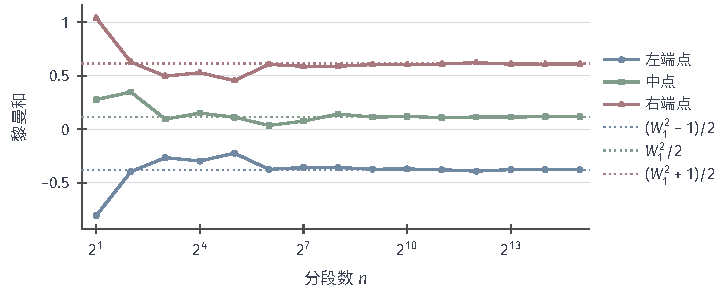
\includegraphics[width=105mm]{figures/03-optimization-evolution-and-signals/02-processes-and-trajectory-evolution/tikz/ctsp-ito-stratonovich-sums/figure.pdf}
  \caption{同一条Brownian教学路径（$2^{16}$个增量，固定随机种子）上$\int_0^1W\,\mathrm dW$的三种Riemann和，横轴为二进分割的段数。左端点、中点、右端点取样分别趋向$(W_1^2-1)/2$、$W_1^2/2$与$(W_1^2+1)/2$（同色点线）。左端点对应Itô积分，中点对应Stratonovich积分；两者之差是二次变差的一半，并非网格误差。}
  \label{fig:ctsp-ito-stratonovich-sums}
\end{figure}

左端点取样的优点是被积系数不偷看本段增量，从而保留鞅性质与等距；代价是普通链式法则需要修正。中点或两端平均取样恢复了普通链式法则，但失去了鞅性质：$\mathbb E\frac12W_1^2=\frac12\neq0$。两种约定各有用途，关键是在建模时说清用的是哪一种。

\paragraph{连续半鞅上的Stratonovich积分}
把有限变差部分与连续局部鞅之和称为\term{连续半鞅}（continuous semimartingale）；Itô过程都是连续半鞅。对连续半鞅$H$与$X$，定义
\begin{equation}
  \int_0^tH_s\circ\mathrm dX_s=\int_0^tH_s\,\mathrm dX_s+\frac12[H,X]_t ,
  \label{eq:ctsp-stratonovich}
\end{equation}
称为\term{Stratonovich积分}（Stratonovich integral）。它是两端平均取样$\sum_i\frac12(H_{t_i}+H_{t_{i+1}})\Delta X_i$的依概率极限：与左端点和相比，多出的$\frac12\sum_i\Delta H_i\Delta X_i$正收敛到$\frac12[H,X]_t$。

普通链式法则在这一约定下恢复。设$F\in C^3$，由Itô公式，
\[
  F(X_t)-F(X_0)=\int_0^tF'(X_s)\,\mathrm dX_s+\frac12\int_0^tF''(X_s)\,\mathrm d[X]_s .
\]
另一方面，$F'(X)$本身是连续半鞅，其鞅部分为$\int F''(X)\,\mathrm dM$（$M$是$X$的鞅部分），所以$[F'(X),X]_t=\int_0^tF''(X_s)\,\mathrm d[X]_s$。代入式~\eqref{eq:ctsp-stratonovich}，得到$F(X_t)-F(X_0)=\int_0^tF'(X_s)\circ\mathrm dX_s$，与普通微积分形式相同。需要$C^3$是为了让$F'(X)$可以再用一次Itô公式。

\paragraph{同一模型的两种写法}
Stratonovich记号写出的方程可以改写为Itô方程，但漂移必须修正。对标量模型$\mathrm dX_t=b_{\mathrm S}(X_t)\,\mathrm dt+\sigma(X_t)\circ\mathrm dW_t$，其中$\sigma\in C^2$，由定义有$\sigma(X)\circ\mathrm dW=\sigma(X)\,\mathrm dW+\frac12\mathrm d[\sigma(X),W]$，而$[\sigma(X),W]_t=\int_0^t\sigma'(X_s)\sigma(X_s)\,\mathrm ds$。于是它等价于
\begin{equation}
  \mathrm dX_t=\Bigl[b_{\mathrm S}(X_t)+\tfrac12\sigma(X_t)\sigma'(X_t)\Bigr]\mathrm dt+\sigma(X_t)\,\mathrm dW_t .
  \label{eq:ctsp-strat-to-ito}
\end{equation}
多维时，第$i$个分量的修正为$\frac12\sum_{j,k}\sigma_{k,j}\partial_k\sigma_{i,j}$。加性噪声（$\sigma$为常数）时修正为零，两种写法给出同一个方程。

\begin{example}[乘性噪声的两种解读]
  \label{ex:ctsp-multiplicative-two-readings}
  考虑$\mathrm dX=aX\,\mathrm dt+\sigma X\circ\mathrm dW$，$X_0=x_0>0$。按Stratonovich约定，普通链式法则可用于$\log X$：$\mathrm d\log X=a\,\mathrm dt+\sigma\circ\mathrm dW$，所以$X_t=x_0\exp(at+\sigma W_t)$，路径的平均指数增长率为$a$。由式~\eqref{eq:ctsp-strat-to-ito}，它等价于Itô方程$\mathrm dX=(a+\sigma^2/2)X\,\mathrm dt+\sigma X\,\mathrm dW$。反过来，若把同样的符号理解为Itô方程$\mathrm dX=aX\,\mathrm dt+\sigma X\,\mathrm dW$，下一节将算出$X_t=x_0\exp((a-\sigma^2/2)t+\sigma W_t)$，增长率变为$a-\sigma^2/2$。取$a=0.05$、$\sigma=0.4$，一个模型的典型路径以$0.05$的速率增长，另一个以$0.03$的速率衰减。两种约定之间的转换保持的是同一个随机模型，单纯更换积分记号而不修改漂移，会把模型换成另一个。
\end{example}

哪种约定更适合建模，取决于噪声的来源。若真实的扰动是相关时间很短的光滑噪声，用它驱动普通微分方程，再让相关时间趋零，在适当条件下极限是Stratonovich方程（Wong--Zakai型结果）\scite{math-oksendal2003sde}；若噪声来自离散时刻独立的冲击，而系数在冲击前确定，Itô约定更自然。有跳跃时，对称取样的约定还要另行规定跳跃处的取值，本章不进入这一情形。
